\documentclass[a4paper, 12pt]{scrartcl}
\usepackage{geometry}
\usepackage[utf8x]{inputenc}
\usepackage[ngerman]{babel}
\usepackage[parfill]{parskip}
\usepackage{float}
\usepackage{hyperref}
\usepackage{tikz}
\usepackage{tabulary}

%packages für grafiken
\usepackage{graphicx}
\usepackage{placeins}
\usepackage{capt-of}

\title{Power-over-Ethernet SNMP Diagnose Tool}
\subtitle{Computer Networks - Group 1}
\author{Roman Khassraf (0827800)\\ Felix Mayerhuber (0825283) \\ Christopher Morrent (0925960) \\ Christoph Wachter }
\date{\today}

\begin{document}

\maketitle

\section{Einführung}
\label{sec:intro}
Die vorliegende Arbeit beschäftigt sich mit der Überwachung von Switches, die Endgeräte über die Datennetzverkabelung mit Strom versorgen. Die Stromversorgung erfolgt dabei über die Technologie Power-over-Ethernet (PoE), die in Abschnitt \ref{sec:poe} detaillierter beschrieben wird. Die Vorteile dieser Methode liegen in der Ersparnis von Stromverkabelung sowie in der Möglichkeit der Steuerung der Energieversorgung. PoE nutzt dabei die zur Netzwerkanbindung notwendige Ethernet-Verkabelung zur Energieversorgung der Endgeräte.

Der Einsatz dieser Methode bringt jedoch auch Einschränkungen mit sich. Die Leistung, die ein Switch zur Verfügung stellen kann, ist von der Technologie limitiert. Je nach verwendetem Standard ist die Leistung je Port auf 15,4-60 Watt beschränkt. Auch die gesamte Versorgungsleistung, die ein Switch zur Verfügung stellen kann, ist begrenzt. Die Gesamtleistung ist dabei vom Switchtyp abhängig. 

Bei einem großflächigen Einsatz von PoE ergibt sich aus diesen Einschränkungen die Notwendigkeit, die Leistungsabgabe der Switches zu überwachen. Verschiedene Parameter sind von besonderem Interesse für den Betrieb dieser Technologie. Dies sind zum Beispiel die Leistungsaufnahme einzelner Endgeräte, die gesamte abgegebene Leistung eines Switch, die Veränderung der Werte im Laufe des Betriebs und die verfügbare Leistung für weitere Endgeräte.

Mit dem Simple Network Management Protocol (SNMP), das in Abschnitt \ref{sec:SNMP} beschrieben ist, steht eine bewährte und weit verbreitete Technologie zur Verfügung, die ein regelmäßiges Auslesen von Informationen über ein standardisiertes Protokoll erlaubt. Es ermöglicht damit Zugriff auf jene Informationen der implementierenden Netzwerkkomponente, die diese über SNMP zur Verfügung stellt. Die Definition der verfügbaren Informationen erfolgt in der Management Information Base (MIB). Mit Hilfe von SNMP können die für die zuvor erwähnte Überwachung notwendigen Daten aus einem Switch abgerufen werden, sofern dieser SNMP implementiert und die für die Überwachung des PoE-Betriebs relevanten Daten verfügbar macht.

Die Zielsetzung der vorliegenden Arbeit ist es, ein Werkzeug zu entwickeln, mit dessen Hilfe die für den Betrieb von PoE relevanten Daten über einen längeren Zeitraum gesammelt werden können. Die Daten stehen somit für weitere Auswertungen zur Verfügung, um als Entscheidungsgrundlage für das Management des Betriebs zu dienen. Dabei konzentriert sich die Arbeit auf PoE-fähige Switches des Herstellers Cisco, wobei eine Einschränkung auf die beiden Typen WS-C3560G-24PS-S und WS-C2960S-48FPS-L erfolgt. Vorbereitend werden jene Informationen identifiziert, die von den beiden Switchtypen verfügbar gemacht werden können und für die Zielsetzung relevant sind. In weiterer Folge wird eine Software entwickelt, die die ausgewählten Informationen in regelmäßigen Abständen abruft. Dabei findet das bereits erwähnte SNMP Verwendung. Die Daten werden in der Software visualisiert, und können für eine weitere Verarbeitung in einem standardisierten Format exportiert werden.

\section{Grundlagen}
\label{sec:basics}

In dieser Sektion werden die Technologien, welche die Grundlage für das Monitoring Tool darstellen, kurz erläutert. Für jede dieser Technologien wird die Motivation und die grundsätzliche Funktionalität erklärt.

\subsection{Power-over-Ethernet (PoE)}
\label{sec:poe}
Mit Power-over-Ethernet (PoE) ist es möglich, dass man Geräte über die oft schon vorhandenen Netzwerkkabel mit Strom versorgen kann. Die Idee dahinter, warum man sich überhaupt darüber Gedanken gemacht hat, war dass es eine Menge Geräte gibt die eigentlich eine geringe Stromversorgung brauchen, diesen Strom jedoch durch einen Anschluss an der Stromversorgung des Gebäudes tilgen. Was bedeutet: Überall wo man einfache Netzwerkgeräte braucht (Print-Server, Voice-over-IP Geräte, etc.) braucht man immer sowohl Netzwerk- als auch Stromkabel.

Mittels PoE können die zusätzlichen Stromkabel eingespart werden, sofern das Gerät eine Ladung über das Netzwerk-Interface erlaubt. Dies eignet sich sehr gut für einige eher einfache Geräte wie Webcams, Handhelds, etc.

Für PoE wurden bisher zwei IEEE Standards verabschiedet. Tabelle \ref{tab:compareIeee} zeigt einen kurzen Vergleich zwischen den beiden Standards.

\begin{table}[h]
 \centering
 \begin{tabular}{|c|c|c|c|}
   \hline
   \textbf{IEEE Nummer} & \textbf{Bezeichnung} & \textbf{Leistung / Port} & \textbf{nutzbare Leistung} \\
   \hline
   IEEE 802.3af & PoE & 15,4 Watt & ca. 12,9 Watt \\
   \hline
   IEEE 802.3at & PoE+ & 60 Watt & ca. 51 Watt \\
   \hline
 \end{tabular}
 \caption{Vergleich IEEE Standards \cite{poe2}}
 \label{tab:compareIeee}
\end{table}

Die nutzbare Leistung unterscheidet sich deshalb von der Leistung / Port, weil hier auch der Verlust der bei den RJ-45 Steckern passiert und auch den Verlust über eine Strecke von 100 Metern eingerechnet wurde.

\subsubsection{IEEE 802.3af}
Dieser Standard funktioniert nur mit 10Base-T und 100Base-TX Verbindungen. Die Idee hinter diesem Standard ist, dass man die freien Aderpaare (bei diesen beiden Verbindungen werden nur 2 der 4 Paare verwendet) für die Stromübertragung verwendet. Dieses Verfahren wird \emph{Spare-Pairs-Verfahren} genannt. Abbildung \ref{fig:spare-pairs} zeigt den Aufbau dieses Verfahrens.

\begin{figure}[h]
    \centering
    \leavevmode
    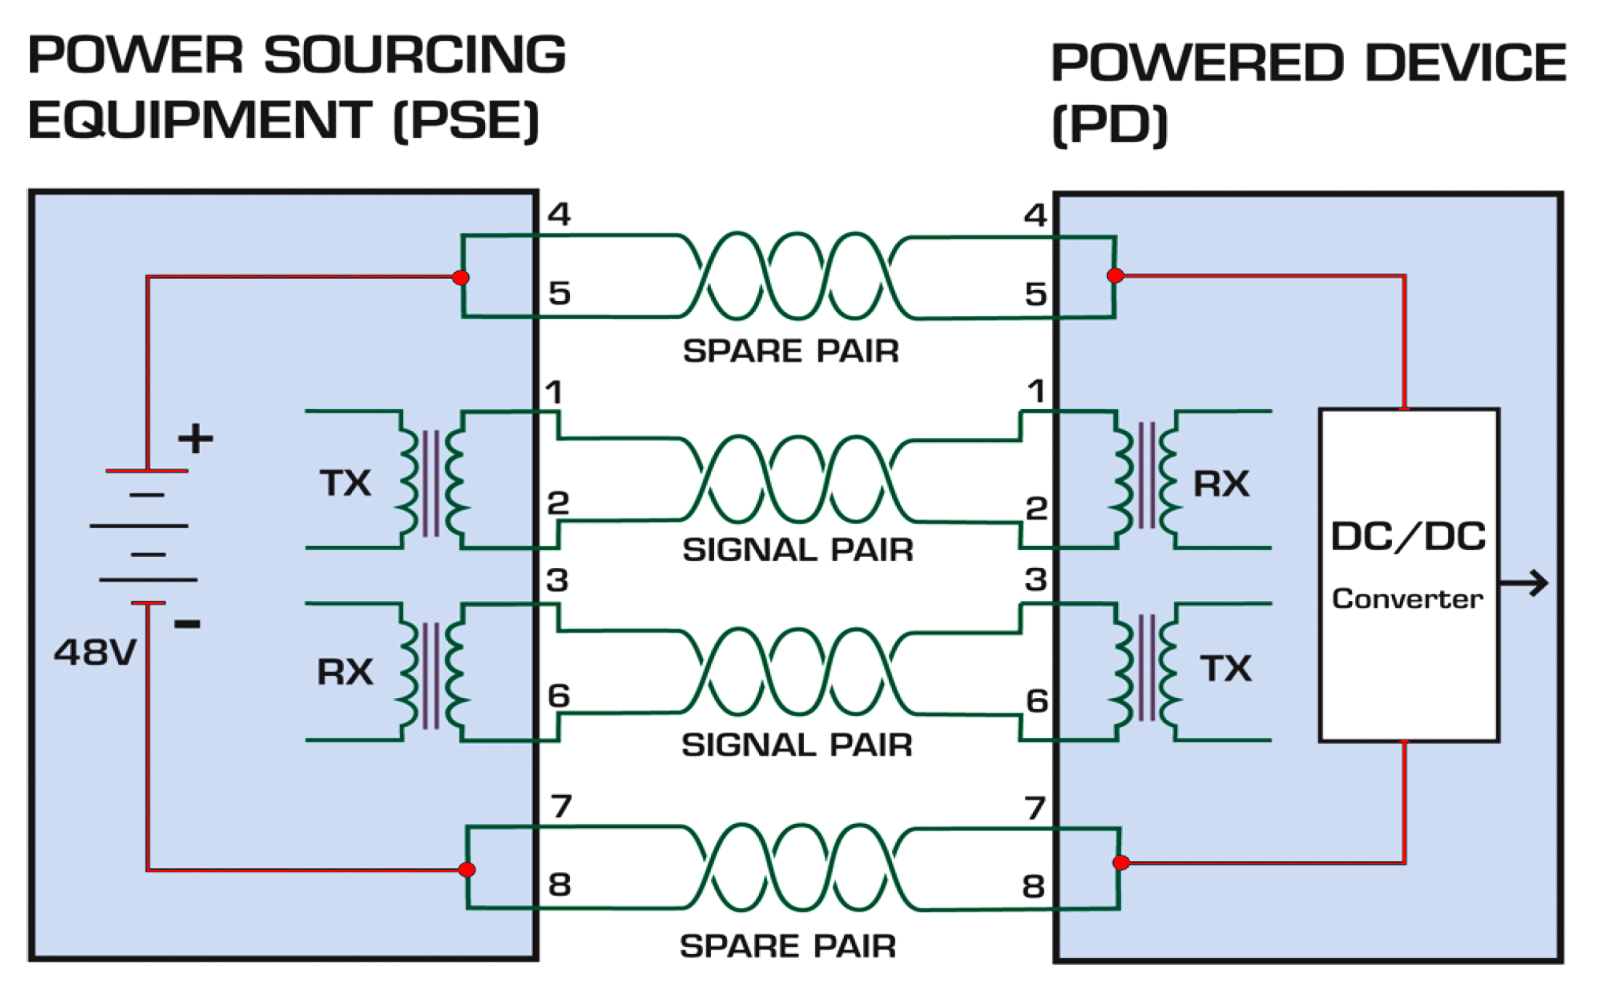
\includegraphics[width=1.0\linewidth]{figures/spare-pairs-verfahren-marked}
    \caption{Spare-Pairs-Verfahren\cite{poe1}}
    \label{fig:spare-pairs}
\end{figure}

Es gibt diesen Standard in verschiedenen Klassen. Die Default Klasse entspricht den oben beschriebenen Spezifikationen. Die anderen Klassen können teilweise auch mehr Leistung bereit stellen (bis zu ca. 21 Watt). Es gibt auch Switches, welche ca. 30 Watt pro Port bereit stellen, diese verhalten sich jedoch nicht dem Standard entsprechend.

\subsubsection{IEEE 802.3at}
Dieser Standard ist auch bei 1000Base-T Verbindungen anwendbar. Hier wird der Strom nicht in den unbenutzten Aderpaaren übertragen (die gibt es hier ja nicht), sondern der Strom wird mit dem übertragenen Daten überlagert und somit parallel übertragen. Dieses Verfahren wird \emph{Phantom-Speisung} genannt. Abbildung \ref{fig:phantom-speisung} zeigt den Aufbau dieses Verfahrens.

\begin{figure}[h]
    \centering
    \leavevmode
    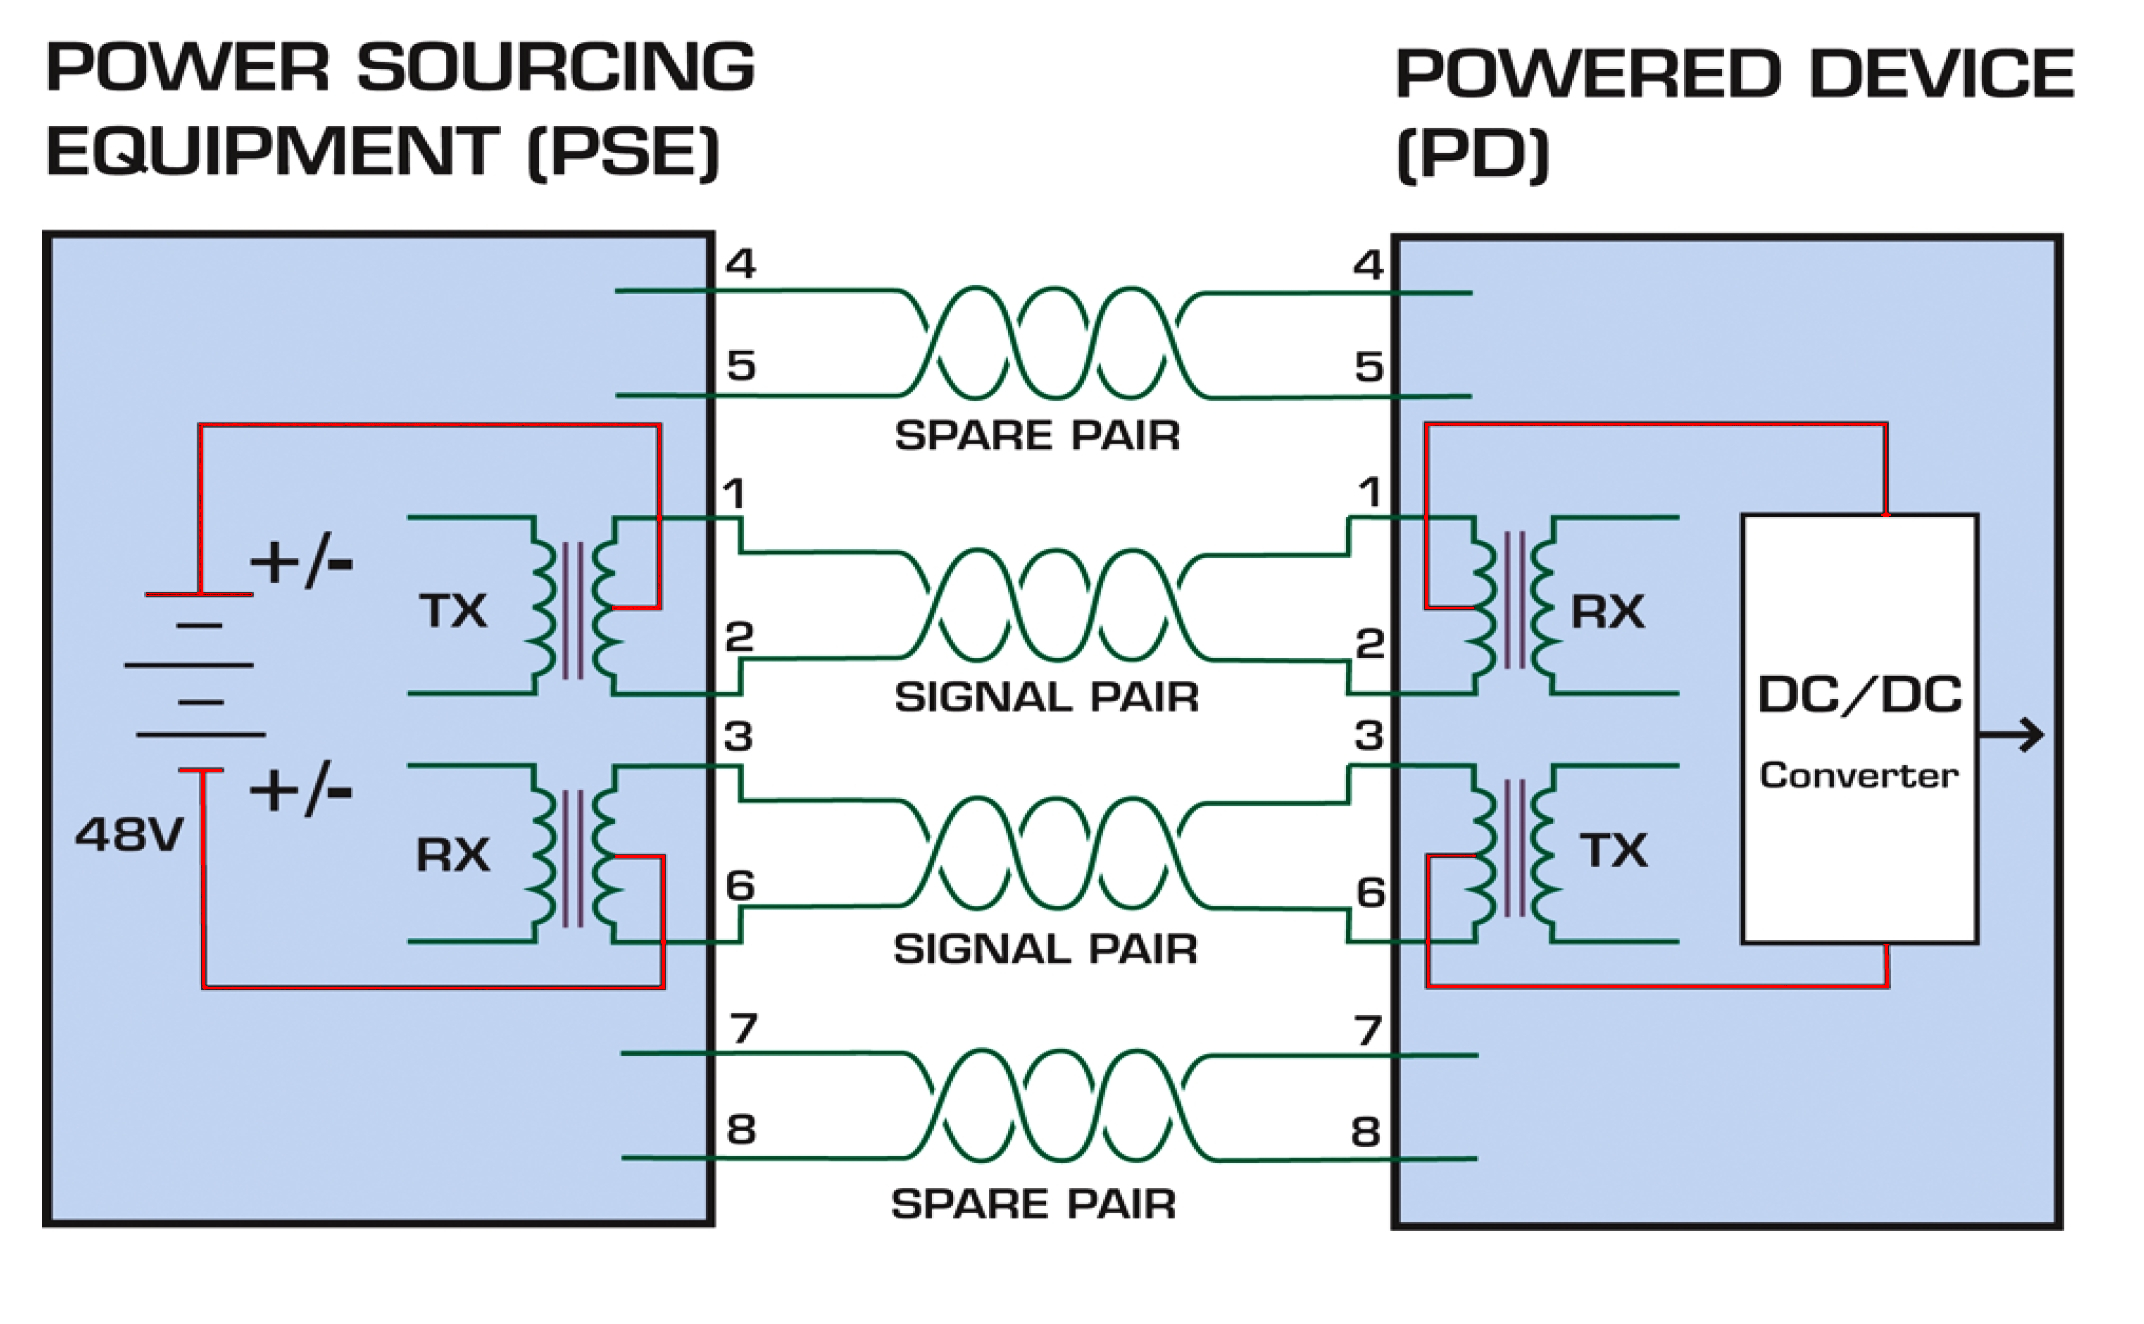
\includegraphics[width=1.0\linewidth]{figures/phantom-speisung-marked}
    \caption{Phantom-Speisung \cite{poe1}}
    \label{fig:phantom-speisung}
\end{figure}

Dieser Standard bietet höhere nutzbare Leistung, braucht aber auch bessere Kabel um richtig zu funktionieren.

\subsubsection{Energieversorgung}

Für die Versorgung der Kabel mit Strom, um sie beim Empfänger benutzen zu können, gibt es zwei Möglichkeiten\cite{poe2}:
\begin{description}
 \item[Endspan -] Es gibt direkt einen Switch welcher die Ports mit Energie versorgt.
 \item[Midspan -]Man baut auf halber Strecke (deshalb Midspan) ein zusätzliches Gerät in das Netzwerk ein, welches die Leitung mit Energie versorgt. Dies ist notwendig, solange man PoE in einen Bereich einsetzen will, in dem es noch keine PoE-fähigen Switche gibt. Das zusätzlich installierte Gerät wird auch Injector genannt.
\end{description}

Wichtiger Punkt hier ist noch, dass ein PoE Switch keine Geräte beschädigen darf, die angeschlossen sind, jedoch kein PoE unterstützen. Hierfür ist es notwendig, dass der PoE Switch erkennen kann ob ein angeschlossenes Gerät mittels PoE mit Energie versorgt werden soll oder nicht. Um dies zu gewährleisten, wurde in den IEEE Standards eine Stufe in der Kommunikationsaufbauphase hinzugefügt.

Hier wird mit kleiner Stromstärke geprüft ob der Empfänger einen gewissen Stromwiderstand hat (die Bereiche sind genau definiert). Falls ja, wird geprüft welcher PoE Standard verwendet werden soll. Danach beginnt die Speisung mit Strom und die Datenverbindung wird aufgebaut.

\subsection{SNMP}
\label{sec:SNMP}
Simple Network Management Protocol (SNMP) ist ein in RFC 1157 definiertes Protokoll zur Überwachung und zum Management von Netzwerkkomponenten.\cite{rfc1157} In RFC 3410 werden Erweiterungen definiert, die als SNMPv3 aktueller De-facto-Standard sind.\cite{rfc3410}

Das Protokoll zielte darauf ab, eine schnell zu implementierende und einfache Lösung für das Management von Netzwerkkomponenten zu erhalten. Bei der Definition von SNMP wurden daher Abstriche beispielsweise hinsichtlich der Sicherheit in Kauf genommen. In SNMPv3 wurden diesbezüglich einige Verbesserungen vorgenommen.

Bei SNMP wird zwischen zwei Entitäten unterschieden, Manager und Agents. Manager, oft auch als Network Management Stations (NMS) bezeichnet, sind für das Abrufen und Empfangen von Informationen über SNMP verantwortlich.\cite{essential-SNMP} Agents sind Software-Artefakte, die auf den Netzwerkkomponenten ausgeführt werden. Ihre Aufgabe ist es, Managern Daten zur Verfügung zu stellen oder diese an die Manager zu senden. Abfragen des Managers an den Agent werden als Query bezeichnet. Unter Trap versteht man eine asynchrone Übermittlung des Agenten an den Manager, nachdem der Agent den Eintritt eines vordefinierten Ereignisses festgestellt hat. Bild \ref*{fig:snmp-schema} stellt die Beziehung der beiden Enitäten zu einander schematisch dar.

\begin{figure}[tbph]
\centering
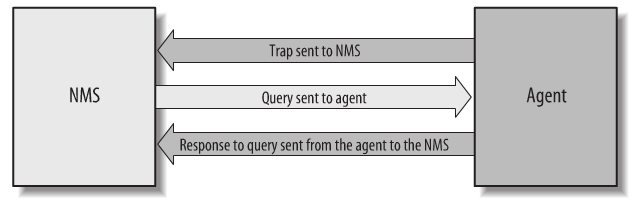
\includegraphics[width=0.7\linewidth]{./figures/snmp-schema}
\caption{Schema der Manager/Agent-Beziehung, aus \cite{essential-SNMP}}
\label{fig:snmp-schema}
\end{figure}

Die vom Agent verfügbar gemachten Daten sind in als Baum aufgebauten Datenbanken, den sogenannten Management Information Base(s) (MIB), definiert. Ein Agent kann dabei mehrere MIBs implementieren.\cite{essential-SNMP} Die Informationen stehen dabei in den Blättern des Baums zur Verfügung. Die Knoten dienen zur Organisation des Baums. Der Zugriff auf ein Blatt erfolgt anhand von eindeutigen Object Identifiern (OID), die einen Pfad im Baum zum gewünschten Blatt darstellen. Abbildung \ref{fig:snmptree} zeigt beispielhaft, wie ein solcher Baum aussehen könnte. In diesem Baum gibt es insgesamt sechs Blätter, es kann somit auf sechs Daten zugegriffen werden. Die OID 1.3.17.18 verweist hierbei auf das mittlere Blatt des rechten Astes. Neben den OIDs werden in MIBs weitere Informationen wie zum Beispiel ein sprechender Name und ein Datentyp für das jeweilig beschriebene Objekt festgelegt.

\begin{figure}[H]
  \begin{center}
    \begin{tikzpicture}[level/.style={sibling distance=30mm/#1}]
      \node [circle,draw] {$1$}
        child {node [circle,draw] {$1$}}
        child {node [circle,draw] {$2$}
          child {node [circle,draw] {$1$}}
          child {node [circle,draw] {$2$}}
        }
        child {node [circle,draw] {$3$}
          child {node [circle,draw] {$17$}
            child {node [circle,draw] {$1$}}
            child {node [circle,draw] {$18$}}
            child {node [circle,draw] {$19$}}
         }
       };
    \end{tikzpicture}
    \caption{Beispiel eines MIB Baumes}
    \label{fig:snmptree}
  \end{center}
\end{figure}

Die Kommunikation zwischen Manager und Agent erfolgt über Protocol Data Units (PDUs), die das Nachrichtenformat der Kommunikation festlegen.\cite{essential-SNMP} Die wichtigsten fünf PDUs sind die folgenden:

\begin{description}
  \item[GET REQUEST:] Anfrage des Managers an den Agent. Der Agent beantwortet die Anfrage mit einem \textbf{GET RESPONSE}.
  \item[GET RESPONSE:] Antwort eines Agents auf eine Anfrage.
  \item[SET REQUEST:] Manager fordert einen Agent zur Änderung eines Wertes auf. Als Antwort erhält der Manager ein \textbf{GET RESPONSE} vom Agent. Im Fehlerfall wird dem Manager darin ein Fehlercode übermittelt.
  \item[GET\_NEXT REQUEST:] Manager forder jenen Wert im Baum an, der als nächstes aufgelistet ist. Dabei wird eine Tiefensuche angewendet. Der Agent beantwortet die Anfrage mit einem \textbf{GET RESPONSE}. Hierbei ist jedoch zu beachten, dass dieser Wert nicht zwingend der tatsächlich gewünschte Wert ist. Existiert das gewünschte Blatt nicht, liefert die Anfrage trotzdem das Datum des nächsten Knotens.
  \item[TRAP:] Im Eintrittsfall eines vordefinierten Ereignisses sendet der Agent an einen zuvor konfigurierten Manager eine Nachricht. Der Agent erhält hierbei keinerlei Bestätigung über den Empfang der Trap.
\end{description}


\section{Switches und SNMP-MIB}
\label{sec:cisco}

Die f\"ur die vorliegende Arbeit verwendeten Switchtypen von Cisco sind ein 24 Port Gigabit Switch des Typs WS-C3560G-24PS-S, sowie ein 48 Port Gigabit Switch des Typs WS-C2960S-48FPS-L. Beide Switchtypen werden \"ublicherweise im Access-Bereich eingesetzt und unterst\"utzen folgende PoE-Standards bzw. Protokolle:
\begin{description}
\item[Cisco pre-standard powered devices:] Cisco-propriet\"ares Protokoll, welches das Cisco Discovery Protocol verwendet um den Switch mitzuteilen, dass das Endger\"at PoE-f\"ahig ist. Wird zum Beispiel von Ciscos IP Telefonen oder Access Points verwendet.
\item[Cisco intelligent power management:] Ist ebenso ein Cisco-propriet\"ares Protokoll und eine erneuerte und erweiterte Version von \emph{Cisco pre-standard powered devices}.
\item[IEEE 802.3af]
\item[IEEE 802.3at:] Auch als PoE+ bezeichnet. Au{\ss}erdem wird Universal Power over Ethernet, eine Cisco-propriet\"are Erweiterung des Standards, f\"ur bis zu 60 Watt Versorgungsleistung pro Port, unterst\"utzt.
\end{description}

\subsection{Endger\"ate-Erkennung und initiale Leistungszuweisung}
Da die Switches jedoch nicht gleichzeitig die maximal m\"ogliche Wattanzahl auf allen Ports bereitstellen k\"onnen, ist ein umfangreiches Power-Management notwendig. Die Switches stellen daf\"ur ein globales PoE-Power-Budget zur Verf\"ugung. Die Gr\"o{\ss}e des Budgets ist dabei abh\"angig vom Switchtyp und der Portanzahl. Bei den uns zur Verf\"ugung gestellten Switchtypen betr\"agt das Power-Budget 370 Watt (WS-C3560G-24PS-S)\cite{cisco-c3560g-datasheet} sowie 740 Watt (WS-C2960S-48FPS-L)\cite{cisco-c2960s-datasheet}.

Bei Anschluss eines PoE-Endger\"ates erkennen die Switches ein Cisco pre-standard kompatibles bzw. nach IEEE 802.3-Standard kompatibles Endger\"at, wenn der jeweilige Port PoE-f\"ahig ist, nicht administrativ deaktiviert wurde, PoE am Port aktiviert ist (dies ist standardm\"a{\ss}ig der Fall) und das angeschlossene Endger\"at nicht bereits mittels Netzteil versorgt wird. Sind diese Bedingungen erf\"ullt, wird bei Anschluss eines PoE-Ger\"ats an einen PoE-Port folgenderma{\ss}en eine initiale Leistungszuweisung aus dem Globalbudget des Switches dem Port zugewiesen:
\begin{itemize}
\item [-] im Falle eines Cisco pre-standard Endger\"ats: 15,4 Watt (Bzw. 30 Watt wenn der Switch PoE+-f\"ahig ist.)
\item [-] im Falle eines Endger\"ats welches die IEEE-Standards 802.3af u. 802.3at unterst\"utzt, nach der Leistungsklassifikation des Standards, abgebildet in Tabelle \ref{tab:ieeepowerclassifications}.
\begin{table}[h]
 \centering
 \begin{tabular}{|c|c|}
   \hline
   \textbf{Klasse} & \textbf{Max. Speiseleistung} \\
   \hline
   0 (default) & 15,4 Watt \\
   \hline
   1 & 4 Watt \\
   \hline
   2 & 7 Watt \\
   \hline
   3 & 15,4 Watt \\
   \hline
   4 & 30 Watt \\
   \hline
 \end{tabular}
 \caption{IEEE Power Classifications \cite{poe2}}
 \label{tab:ieeepowerclassifications}
\end{table}
\end{itemize}

Bei Ver\"anderung der Portbelegung sowie in einem regelm\"a{\ss}igen Intervall \"uberpr\"uft der Switch, ob sich die Leistungsanforderungen der Endger\"ate ge\"andert haben und gew\"ahrt oder verweigert die Leistungsanforderungen der Endger\"ate je nach vorhandenem Power-Budget.

\subsection{Power Management Modi}
\label{subsec:power-management-modes}
Die beiden Switchtypen unterst\"utzen die folgenden Power Management Modi bezogen auf einzelne PoE-Ports:
\begin{description}
\item [auto:] Der Switchport erkennt automatisch ob das angeschlossene Endger\"at PoE-f\"ahig ist und gew\"ahrt oder verweigert die Leistungsanfrage entsprechend dem verf\"ugbarem Power-Budget. F\"ur die Leistungszuweisung an die Endger\"ate gilt hierbei die first-come-first-served Regel. Der auto-Mode ist standardm\"a{\ss}ig auf allen PoE-Ports aktiviert.
\item [static:] Die Switchports in diesem Power Modus haben bei der Leistungszuweisung Priorit\"at gegen\"uber den Ports im auto-Modus. Ihnen wird die konfigurierte Leistungsanforderung, sofern durch das globale Power-Budget gedeckt, standardm\"a{\ss}ig zugewiesen.
\item [never:] Auf diesen Switchports ist Power over Ethernet deaktiviert. 
\end{description}

\subsection{Power Monitoring mittels SNMP-MIB}
Der Switch misst und sammelt verschiedenste Werte beim PoE-Betrieb und stellt diese durch eine SNMP-MIB, der CISCO-POWER-ETHERNET-EXT-MIB\cite{cisco-poe-ext-mib}, zur Verf\"ugung.
Diese MIB ist auch in dieser Arbeit von zentraler Bedeutung, da alle notwendigen Leistungsdaten durch diese MIB ausgelesen werden k\"onnen.

Diese MIB stellt eine gro{\ss}e Anzahl an PoE-bezogenen Objects zur Verf\"ugung, im folgenden sind aber nur die f\"ur diese Arbeit relevanten OIDs n\"aher erl\"autert. Das \textit{X} in der letzten Stelle der OIDs ist hierbei die jeweilige Portnummer des Switchs, beginnend bei 1.

Relevante OIDs:
\begin{description}
\item[cpeExtPsePortEnable (1.3.6.1.4.1.9.9.402.1.2.1.1.1.X):] Power Management Modus des Ports.
M\"ogliche Werte:
\begin{description}
\item ['1' (auto):] Standardeinstellung der Ports. Weitere Erkl\"arungen in Absatz \ref{subsec:power-management-modes}.
\item ['2' (static):] Leistung fix konfiguriert.
\item ['3' (limit):] Leistung per Konfiguration beschr\"ankt.
\item ['4' (disable):] PoE deaktiviert.
\end{description}

\item[cpeExtPsePortDeviceDetected (1.3.6.1.4.1.9.9.402.1.2.1.3.1.X):] Zeigt, ob ein PoE-f\"ahiges Endger\"at am Port erkannt wurde.
M\"ogliche Werte:
\begin{description}
\item ['1' (true):] PoE-f\"ahiges Endger\"at erkannt
\item ['2' (false):] kein PoE-f\"ahiges Endger\"at erkannt
\end{description}

\item[cpeExtPsePortPwrMax (1.3.6.1.4.1.9.9.402.1.2.1.6.1.X):] Maximal verf\"ugbare Leistung am Port; konfigurierbar (in Milliwatt)
\item[cpeExtPsePortPwrAllocated (1.3.6.1.4.1.9.9.402.1.2.1.7.1.X):] Zugewiesene Leistung am Port (in Milliwatt)
\item[cpeExtPsePortPwrAvailable (1.3.6.1.4.1.9.9.402.1.2.1.8.1.X):] Verf\"ugbare Leistung am Port, kann sich von der zugewiesenen Leistung (\emph{cpeExtPsePortPwrAllocated}) unterscheiden. (in Milliwatt)
\item[cpeExtPsePortPwrConsumption (1.3.6.1.4.1.9.9.402.1.2.1.9.1.X):] Tats\"achlicher Verbrauch des Endger\"ats. (in Milliwatt)
\item[cpeExtPsePortMaxPwrDrawn (1.3.6.1.4.1.9.9.402.1.2.1.10.1.X):] Maximale Leistungsabnahme des angeschlossenen Endger\"ats seit Einschaltung des Endger\"ats. (in Milliwatt)

\end{description}






\section{PoE SNMP Monitoring Tool}
\label{sec:tool}
Diese Sektion beschreibt das durch das Projektteam entwickelte Tool welches für das PoE Monitoring verwendet wird.
Hierfür wird neben der Beschreibung der Oberfläche auch Details über den Aufbau des Tools illustriert.

\subsection{Architektur}

Das PoE-Tool besteht grundsätzlich aus drei Komponenten (beziehungsweise vier wenn man die Datenbank mit zählt), welche in Abbildung \ref{fig:architecture} dargestellt werden. 

\begin{figure}[h]
    \centering
    \leavevmode
    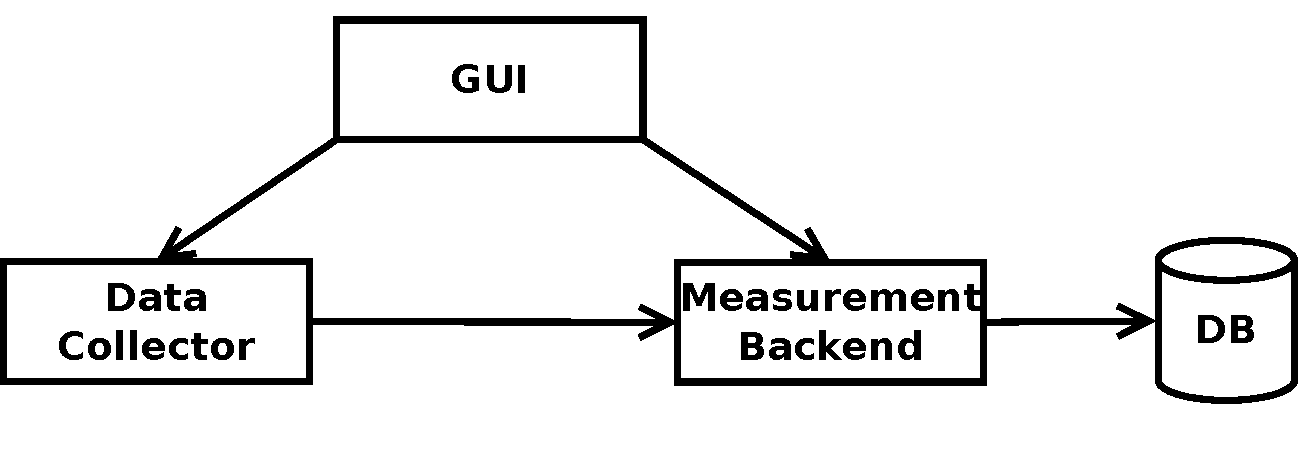
\includegraphics[width=1.0\linewidth]{figures/architecture_new}
    \caption{Software-Architektur PoE SNMP Monitoring Tool}
    \label{fig:architecture}
\end{figure}

Die Funktionen der einzelnen Komponenten ist wie folgt eingeteilt:

\begin{description}
  \item[Measurement Backend:] Diese Komponente bildet die Schnittstelle des Systems zu der Datenbank welche für die Speicherung der Nutzdaten des Tools verwendet wird. Diese Komponente bietet Funktionen zum Anlegen, Speichern und Löschen von Switches, Speichern von Messungen und dem Abfragen dieser durch verschiedenste Kriterien.
  \item[Data Collector:] Diese Komponente ist für die kontinuierliche Abfrage (die Intervalle werden im Config-File angegeben) von Messungen für alle aktiven Switches verantwortlich. Während jeder Messung wird der aktuelle PoE Status jedes Ports pro Switch ausgelesen. Nachdem die Werte aller Ports eines Switches ausgelesen wurden, werden die entsprechenden Messungen an das \textbf{Measurement Backend} zum Speichern eben dieser gesendet.
  \item [GUI] Die GUI-Komponente nimmt Benutzeranfragen entgegen und fragt die darzustellenden Daten vom \textbf{Measurement Backend} ab. Das \textbf{Measurement Backend} liefert die entsprechenden Daten die dann in ein übersichtliches, von Menschen verwertbares, Datenmaterial konvertiert und angezeigt werden.
\end{description}

\subsection{Konfiguration}

Das PoE-Tool wird über die Konfigurationsdatei \textbf{config.properties} angepasst. Diese enthält folgende Optionen:

\begin{description}
  \item [measurement.interval] Dieser Wert gibt die Zeit in Millisekunden an, die zwischen zwei Messungen des selben Switches vergehen sollen. Dieser Wert muss je nach Struktur des Netzwerks gewählt werden, da hier auch die Zeit die der Switch zum Antworten auf SNMP Anfragen braucht eingerechnet werden muss. Ein zu kleiner Wert raubt den Messungen die Aussagekraft.
  \item [distribution.slots] Basierend auf diesem Wert, wird das Zeitintervall, welches in \textbf{measurement.interval} definiert ist, in x Zeitslots eingeteilt. Diese Einstellung wurde eingeführt, damit nicht alle Switches immer zur gleichen Zeit befragt werden und statt dessen eine bessere Verteilung der Anfragen gewährleistet wird. Zum Beispiel: Intervall ist auf 1000 ms und Slots auf 10 eingestellt. Daraufhin wird das Intervall in 10 Slots aufgeteilt, die 100 ms von einander entfernt sind.
  \item [\textbf{data.retriever.impl}] Dieser Wert gibt an welche Implementierung der SNMPDataRetriever, welcher verwendet wird um eine Messung via SNMP durchzuführen. Derzeit gibt es zwei Implementierungen dieses Interfaces:
  \begin{description}
   \item[cn.poe.group1.collector.DummyDataRetriever:] Ist eine Testimplementierung welche das Laden von SMNP Werten nur simuliert und Testwerte zurück gibt. Wurde für die Erstellung des Prototyps verwendet.
   \item[cn.poe.group1.collector.DataRetriever:] Ist die reale Implementierung welcher wirklich SMNP Werte von Geräten abfragt.
  \end{description}
\end{description}

\subsection{Verwendung}
Beim Start des PoE-Tool wird die Datenbank auf existierende Switch Definitionen überprüft. Für jede existierende Definition, wird automatisch mit den Messungen für den entsprechenden Switch begonnen. Danach wird das GUI des Tools gestartet, welche alle existierenden Definitionen in der linken Tabelle anzeigt. Wird ein Switch dort ausgewählt, werden seine Nutzdaten im rechten Feld angezeigt.

Wichtig: Die GUI zeigt immer nur die Messdaten aus einem bestimmten Zeitraum an. Dieser kann im Hauptfenster rechts oben definiert werden. Um die Nutzdaten zu aktualisieren, mus der \textbf{Reload} Button betätigt werden.

\subsubsection{Switch}
Durch die Auswahl eines Switches in der linken Tabelle, werden die entsprechenden Nutzdaten geladen. Hierbei sind die Nutzdaten kategorisch auf zwei Registerkarten aufgeteilt:
\begin{description}
 \item[Ports:] Die Werte in dieser Registerkarte listen die Durchschnittszahlen für die PoE Werte der Ports des gewählten Switches auf. Auf diese Weise kann ein schneller Überblick über alle Ports gewährleistet werden. Dieser Reiter wird immer beim Öffnen eines Switches als Standard angezeigt. Details über die Ports werden in Punkt \ref{sub:ports} genauer erläutert.
 \item[Switch:] Dieser Reiter bietet eine Übersicht über die kumulierten Werte der Ports des gewählten Switches in Form einer Kurve. Somit bietet diese Sicht einen guten Überblick über den PoE Werteverlauf des gesamten Switches und erlaubt eine schnelle Überprüfung der Kapazitätsgrenzen des Switches (siehe Abbildung \ref{fig:overview-switch}).
\end{description}

\begin{figure}[h]
    \centering
    \leavevmode
    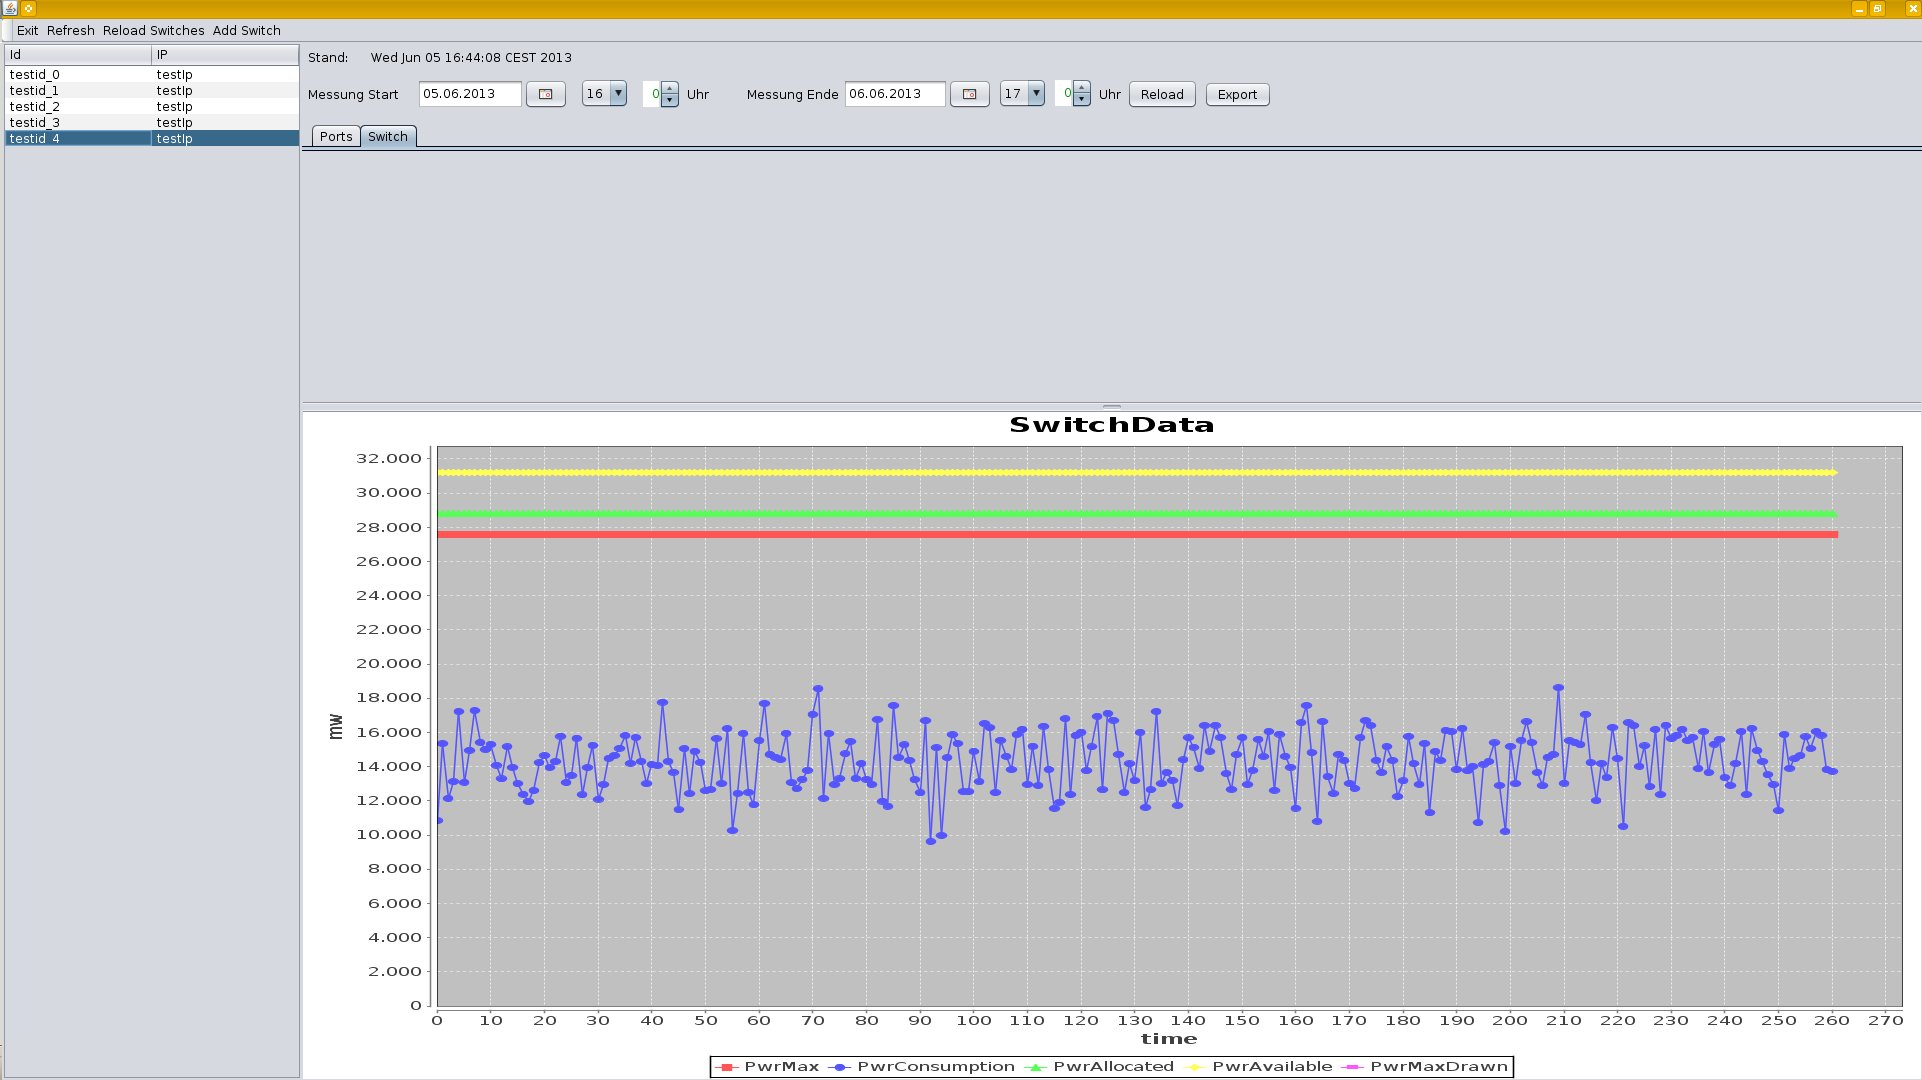
\includegraphics[width=1.0\linewidth]{figures/screenshot2}
    \caption{Übersicht über einen Switch}
    \label{fig:overview-switch}
\end{figure}

Um einen neuen Switch, welcher überwacht werden soll, zu dem Tool hinzuzufügen, gibt es den Menüpunkt \textbf{Add Switch} in der Menüleiste des Tools. Durch aktivieren dieses Menüpunktes, wird ein Popup geöffnet (siehe Abbildung \ref{fig:popup}) welches ausgefüllt und bestätigt werden muss. Nach dem Anlegen eines neuen Switches, beginnen die Messungen automatisch im Hintergrund.

 \begin{figure}[h]
    \centering
    \leavevmode
    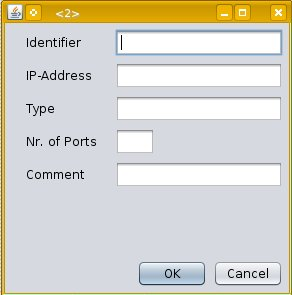
\includegraphics[scale=0.5]{figures/screenshot3.jpg}
    \caption{Popup um neuen Switch anzulegen}
    \label{fig:popup}
\end{figure}

Um Switches editieren beziehungsweise löschen zu können, wurden diese Funktionen in das Kontextmenü der linken Tabelle hinzugefügt. Das Kontextmenü enthält einen Punkt zur Änderung des Switches (\textbf{Edit Switch}) und ein Punkt für das Löschen von Switches (\textbf{Delete Switch}).

\subsubsection{Ports}
\label{sub:ports}
Auf der Registerkarte Port im rechten Teil des Fensters können die Daten über die einzelnen Ports eines Switches betrachtet werden. Die Tabelle enthält dabei einen Mittelwert aus den Messungen über die einzelnen Parameter für den gegebenen Zeitraum. Der Chart enthält einen graphischen Verlauf der einzelnen Parametern. Abbildung \ref{fig:overview-port} zeigt wie die Port Übersicht im Tool aussieht.

\begin{figure}[h]
    \centering
    \leavevmode
    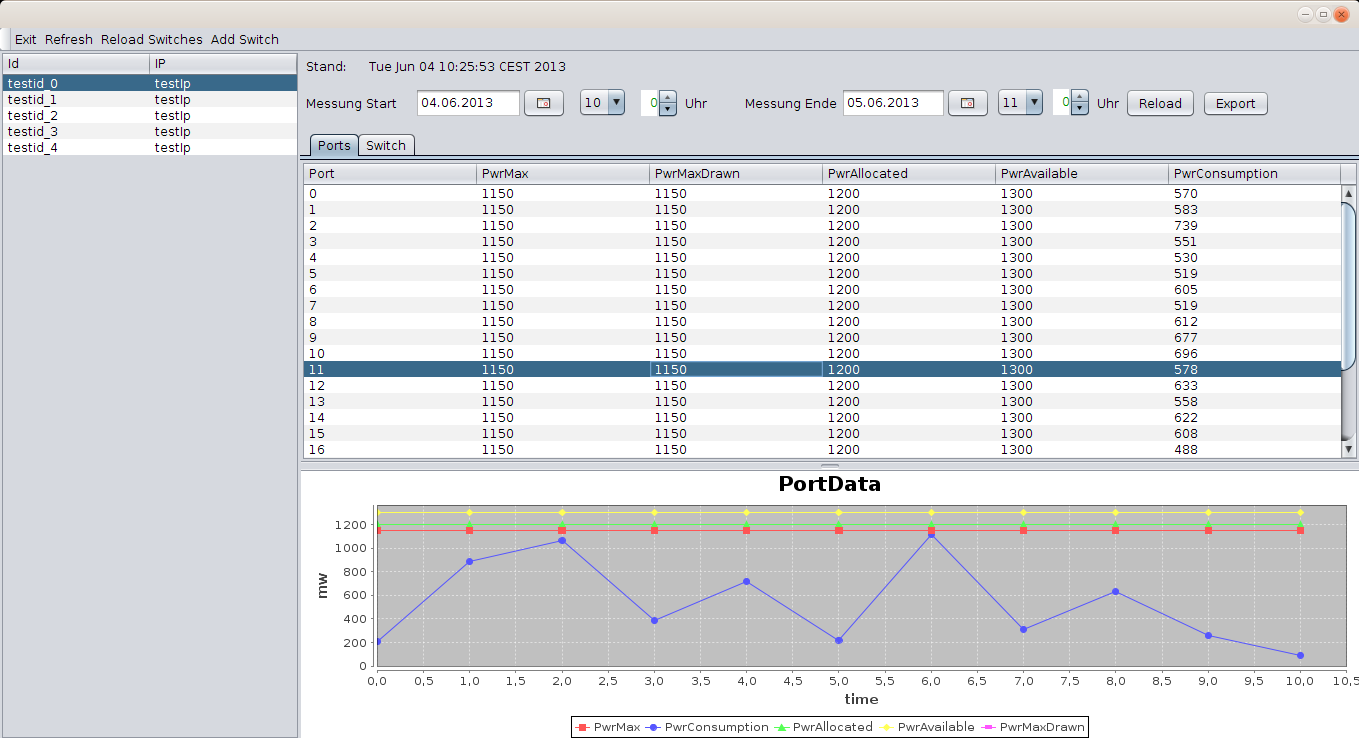
\includegraphics[width=1.0\linewidth]{figures/screenshot1}
    \caption{Übersicht über einen Switch}
    \label{fig:overview-port}
\end{figure}

\subsubsection{CSV Export}
Durch einen Klick auf den Button \textbf{Export} können sämtliche Messungen, welche im angegebenen Zeitraum für den ausgewählten Switch gemacht wurden, in ein CSV-file exportiert werden. Durch betätigen des \textbf{Export} Buttons, wird ein Datei-Dialog angezeigt, in welchen man Ort und Name der resultierenden CSV Datei angeben muss.

\section{Testaufbau \& Ergebnisse}
\label{sec:test}

// TODO: erkläre hier den Testaufbau den wir gehabt haben und wie sich das Tool hier verhalten hat. Eventuell mit ein paar Screenshots mit Realdaten. Hier werden ein paar Seiten zusammenkommen weil wir vermutlich mehrere Tests durchführen (zb. so hat sich das System verhalten mit 3 angesteckten Geräten und so mit 20, ...)

\subsubsection{Testaufbau}
// Welche Switche sind wo? Welche Geräte auf welchen Ports angesteckt.

// Konfiguration vom Tool

\subsubsection{Testablauf}

// Erklärung wie das Ganze abgelaufen ist (Entweder Christopher oder Felix beschreiben das)

In Abbildung \ref{fig:portDetails} sieht man die Auswirkungen durch die Deaktivierung und anschließender Aktivierung eines Ports bezüglich der Werte die durch SNMP erhalten werden. Zwischen der 47 und 48 Messung im Abfragezeitraum wurde das Port per Administration deaktiviert. Augenblicklich fallen die Werte, die mit dem tatsächlichen Verbrauch des Gerätes auf diesen Port zu tun haben, auf 0. 

Bei oder kurz vor Messung 70 wurde das Port wieder aktiviert. Wie man sieht, stieg hierbei der Wert für \textit{PwrAllocated} kurzzeitig auf ein lokales Maximum. Dies liegt daran, dass der Port für den Einschaltvorgang des Gerätes, welches an dem Port hängt, eine höhere Leistung anbieten kann. Kurz darauf normalisiert sich dieser Wert wieder und fällt auf das Mittel (welches vom Switch berechnet wird) zurück.

Auch der tatsächliche Verbrauch steigt von Messung 70 beginnend an auf den Wert den er vor der Abschaltung gehabt hat. Diesen Zustand hat er nach circa 4 Messungen wieder erreicht.

\begin{figure}[h]
    \centering
    \leavevmode
    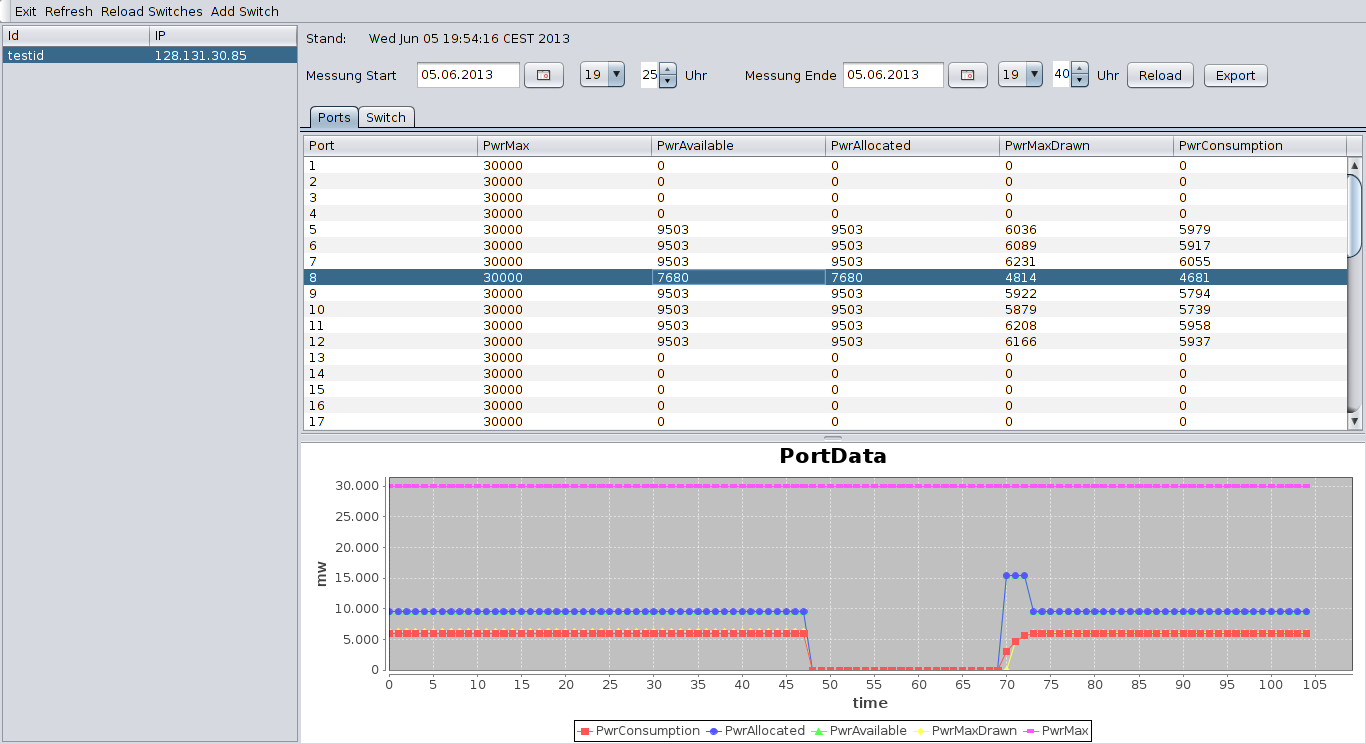
\includegraphics[width=1.0\linewidth]{figures/portDetails}
    \caption{Screenshot Verlauf Port Detail}
    \label{fig:portDetails}
\end{figure}

// Erkläre warum Grafik von Switch so aussieht wie sie aussieht
In Abbildung \ref{fig:switchDetails} sieht man die Auswirkungen durch die Deaktivierung und anschließender Aktivierung der Ports im definierten Testszenario.

\begin{figure}[h]
    \centering
    \leavevmode
    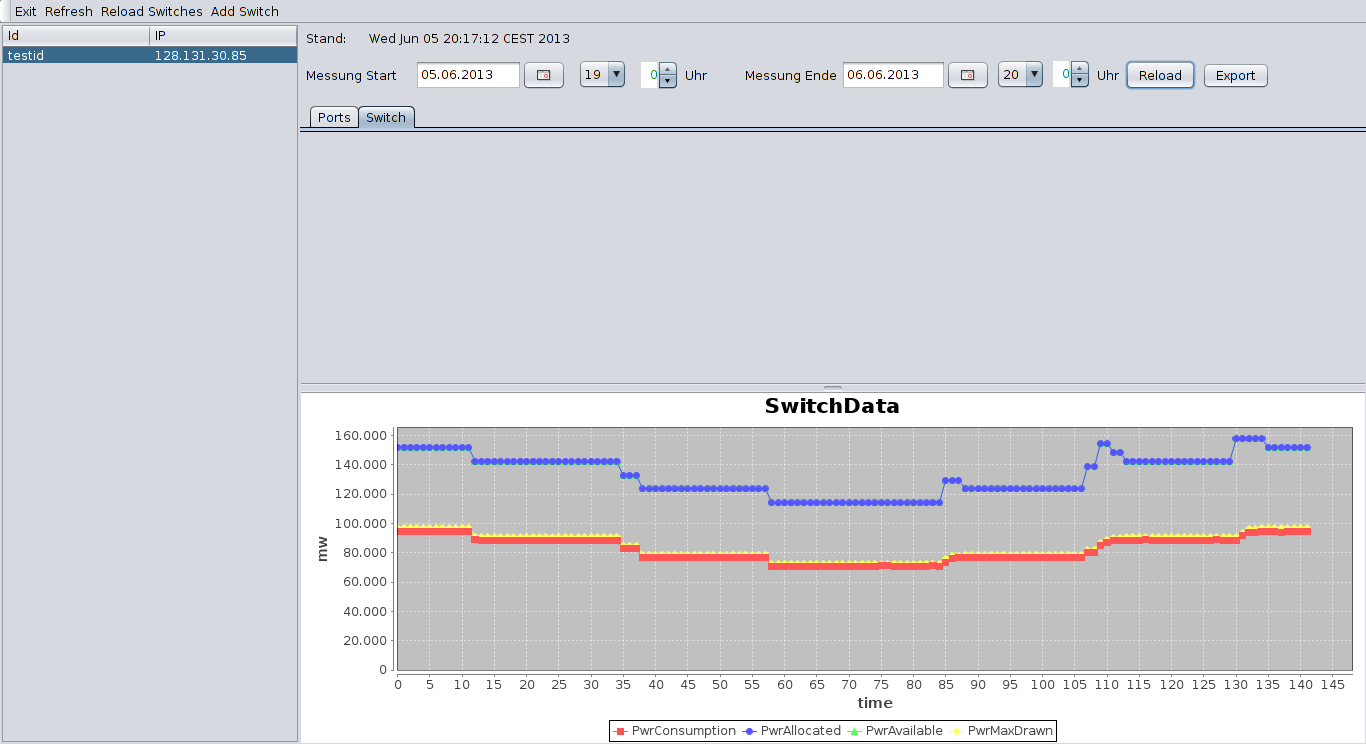
\includegraphics[width=1.0\linewidth]{figures/switchDetails}
    \caption{Screenshot Verlauf Switch Detail}
    \label{fig:switchDetails}
\end{figure}


\begin{thebibliography}{4}

\bibitem{poe1} http://www.scantec.de/knowledge-base/technology-transfer/2007-2/power-over-ethernet-von-akros-silikon.html, letzter Zugriff: 03.06.2013

\bibitem{poe2} http://www.elektronik-kompendium.de/sites/net/0807021.htm, letzter Zugriff: 03.06.2013

\end{thebibliography}


\end{document}





















